\documentclass[11pt]{article}
\usepackage[margin=1in]{geometry}
\geometry{letterpaper}
\usepackage{graphicx}
\usepackage{setspace}
\usepackage{amssymb}
\usepackage{amsmath}
\usepackage{epstopdf}
\usepackage[table,dvipsnames]{xcolor}
\usepackage{color, colortbl}
\usepackage{array}
\usepackage[numbers,sort&compress]{natbib}
\usepackage{fancyhdr}
\pagestyle{fancy}
\fancyhead{}
\fancyhead[LO,LE]{Rominger, {\it et al.}}
\fancyhead[RO,RE]{Project Description}

\usepackage{changepage}

\usepackage{caption, subcaption}
\usepackage{floatrow}

\DeclareCaptionFont{mysize}{\footnotesize}
\captionsetup{font=mysize}


\usepackage[hidelinks]{hyperref}

\usepackage[T1]{fontenc}
\usepackage{titling}
\setlength{\droptitle}{-3.5em}

\usepackage{wrapfig}

\usepackage{multirow}


%% make lists more compact
\usepackage{enumitem}
\setitemize{noitemsep,topsep=0pt,parsep=0pt,partopsep=0pt}
\setenumerate{noitemsep,topsep=0pt,parsep=0pt,partopsep=0pt}


%% make sections, subsections and paragraphs more compact
\makeatletter
\renewcommand\section{\@startsection{section}{1}{\z@}%
                                  {-1.5ex \@plus -1ex \@minus 0.2ex}%
                                  {0.1ex \@plus 0.2ex}%
                                  {\normalfont\Large\bfseries}}
\makeatother

\makeatletter
\renewcommand\subsection{\@startsection{subsection}{1}{\z@}%
                                  {-1.5ex \@plus -1ex \@minus 0.2ex}%
                                  {0.1ex \@plus 0.2ex}%
                                  {\normalfont\large\bfseries}}
\makeatletter

\makeatletter
\renewcommand\subsubsection{\@startsection{subsection}{1}{\z@}%
                                  {-1.5ex \@plus -1ex \@minus 0.2ex}%
                                  {0.1ex \@plus 0.2ex}%
                                  {\normalfont\bfseries}}
\makeatletter

\makeatletter
\renewcommand{\paragraph}{\@startsection{paragraph}{4}{\z@}
  {1.5ex \@plus 1ex \@minus .2ex}{-1em}
  {\normalfont\normalsize\it}
}
\makeatother


% \title{Postdoc Mentoring Plan \vspace{-1.5ex}}
\title{Integrating Across Dimensions of Biodiversity: Developing Novel Theory and Informatics}
\author{}
\date{}


\begin{document}
% \maketitle
% \thispagestyle{fancy} 
% \vspace{-6em}

\section{Intellectual Merit}\label{intellectual-merit}

\subsection{Aims}\label{aims}

As phylogenetic and functional approaches transcend species-based
estimates of diversity, we seek new answers to the age-old question
\cite{Hutchinson1959-ob}, ``What limits diversity?'' At the
intersection of evolutionary history, environmental opportunity,,
functional capacity, and genetic adaptive potential, a suite of
fundamental processes (drift, migration, mutation, speciation,
competition, environmental filtering) and emergent properties
(e.g.~community structure, ecosystem productivity) lead to largely
unexplored feedbacks between species, functional, phylogenetic, and
population genetic diversity. Thanks to initiatives such as NSF's
Dimensions of Biodiversity (DoB) Program, we have gained enough
insight into feedbacks among these multiple dimensions of biodiversity
to know that they complicate previously simple interpretations of
single dimensions. For instance, traits such as body size may directly
shape responses to climate change by impacting population demography,
thus driving biogeographic patterns of lineage distribution, which
themselves define the conditions to which lineages adapt
\cite{Prates2016-gr,Carnaval2014-je}. However, we have yet to to add
complexity to our predictive models of biodiversity and thus not
gained a mechanistic understanding of the interactions among diversity
dimensions. There is now an unprecedented opportunity to advance
understanding of basic and emergent interactions among dimensions, as
rich data describing detailed and large-scale multi-dimensional data
become available through DoB and other similar initiatives.

Because measurements of diversity reflected in the scale of DoB
projects range from small archipelagos to whole biomes, we propose to
synthesize and integrate across projects to understand the general
rules governing biodiversity. Making sense of diverse and
multi-dimensional data within and between such diverse biogeographical
systems requires (1) having the \textbf{informatic ability} to
synthesize and share them and (2) the \textbf{quantitative tools} to
extract insight from synthesized data about the complex,
multi-dimensional processes underlying biodiversity
patterns. \textbf{We propose to fill these two gaps by (1) building an
  open source platform to manage and query diverse streams of
  biodiversity-relevant information, and (2) developing a stochastic
  model of biodiversity that incorporates a range of mechanistic
  processes that jointly predicts species abundance, trait
  distributions, phylogenetic structure, and population genetic
  diversity.}  Through this model we will be able to quantify the
contribution of three distinct classes of processes to the structure
of biodiversity across disparate systems: (i) Stochastic immigration,
speciation and extinction, (ii) species interactions with the biotic
and abiotic environment, and (iii) historical contingencies.

\textbf{To understand the universality of these processes, we will (3)
test our model across five biogeographic systems for which
multi-dimensional biodiversity data are now available,} due largely to
DoB efforts. They include two naturally insular systems with differing
degrees of isolation, age, and adaptive radiation (the Hawaiian island
chronosequence and the marine lakes of Palau) and three forest systems
with key gradients of diversity and evolutionary history, spanning
scales of historic continental disjunctures (the Nearctic forests of
North America and Asia), entire biomes (Amazonia), and large regions of
unique endemism (the coastal Atlantic Forest of Brazil; Fig. 1). The two
island projects additionally afford an explicitly temporal test of our
model's dynamics---via the sediment cores from Palau's marine lakes and
the chronosequence in Hawaii. By selectively augmenting data gathered by
these DoB projects with new field observations, we will be able to test
our model and begin to verify the universality of processes regulating
the diversity of life. The new data we collect with add substantially
to the Tree of Life, particularly for under-sampled clades such as
arthropods and marine invertebrates.

\begin{wrapfigure}[]{r}{0.5\textwidth}
  \label{fig:map} 
  \vspace{-10pt}
  \begin{center}
    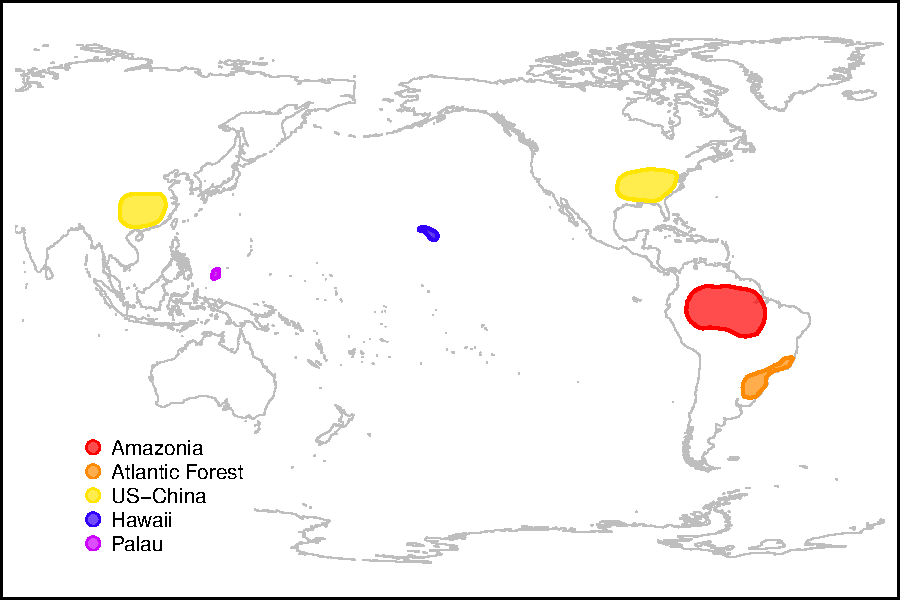
\includegraphics[width=1\textwidth]{../fig_map.pdf}
  \end{center}
  \vspace{-10pt}
  \caption{Map of the included DoB projects showing their breadth of
regions and scales.}
  \vspace{-10pt}
\end{wrapfigure}


\subsection{Background}\label{background}

Understanding the generation and maintenance of biodiversity is critical
to manage and mitigate the effects of anthropogenic change on the
diversity of living systems; without intervention, recovery from the
current crisis \cite{Barnosky2011-ww} could take tens of millions of
years \cite{Erwin2015-yb}. Despite the lack of concrete answers to what
limits diversity, decades of research have generated important insights
into the processes driving diversity across multiple dimensions in
specific systems. Still, mechanistic hypotheses from these studies have
yet to be quantitatively and jointly tested across systems with a
rigorous framework where their universality can be evaluated.

Current eco-evolutionary theory is not up to this task. Quantitative
models inspired by the Equilibrium Theory of Island Biogeography
\cite{MacArthur1967-ux} and the Neutral Theory of Biodiversity and
Biogeography \cite{Hubbell2001-dx}, for instance, place emphasis on the
equilibrium between rates of immigration, speciation, and extinction.Yet
while empirical work on islands and latitudinal gradients have
demonstrated the significant role of immigration, speciation and
extinction histories \cite{Gillespie2004-zv, Owens2017-ja}, these neutral
theories of eco-evolutionary drift are limited. For example,
interspecific interactions and the environment have been shown
empirically to be important in determining patterns such as the
latitudinal diversity gradient
\cite{Janzen1967-fk,Mittelbach2007-ui,Pianka1966-ky}. Moreover, neutral
drift theories do not accurately capture temporal dynamics
\cite{Ricklefs2006-tn, Chisholm2014-mu} and ecological interactions have
been flagged as potential drivers of the fast dynamics observed in real
communities that neutral theories fail to accurately predict
\cite{Rosindell2015-gp,Ricklefs2006-tn}. Conversely, models based on
detailed ecological interactions may be so over-parameterized as to
render them uninterpretable \cite{Rosindell2012-pm}. Current theory
fails to predict multiple dimensions of biodiversity, which can lead to
very different processes producing indistinguishable predictions for
single dimensions
\cite{Chisholm2010-yg,McGill2003-sf,McGill2007-zd,Leibold2017-jv}.

The perspectives from both neutral-like eco-evolutionary drift and
ecological interaction-based coexistence and diversification are
typically applied in equilibrium
\cite{Rominger_undated-cw,Etienne2007-we,Chesson2000-uc,Hubbell2001-dx}.
However, the history underlying a system at any given point might be
such that the system is far from an equilibrium state --something
increasingly relevant in the Anthropocene \cite{Barnosky2012-qz}.
Examples of this non-equilibrium hysteresis include island biogeography
\cite{Ricklefs2001-af}, differences in otherwise similar biomes across
East Asia and North America \cite{Qian2005-co,Yu2017-cc}, and
communities assembled from refugia after climate change
\cite{Carnaval2008-og,Carnaval2009-vd,Burbrink2016-nu}.

Evaluating how general these observations are across systems, and how
they influence species-level, phylogenetic, population genetic, and
functional trait diversity, necessitates the collection, management and
analysis of multi-dimensional data on (i) the abundance of species, (ii)
their geo-referenced occurrences, (iii) ecologically-relevant traits, (iv)
phylogenetic and population genetic histories, and (v) the environment.
We propose to build such informatic synthesis tools and to
quantitatively compare the support for these different hypothesized
mechanisms across five systems.

\subsubsection{Informatic platform for dimensions of biodiversity
data}\label{informatic-platform-for-dimensions-of-biodiversity-data}

Large scale, system-based collaborative projects - including many funded
by the DoB program - often have difficulty making the best use of the
volume and types of data they generate. Data management strategies are
usually developed independently by each team or laboratory, often
varying across teams. Members of collaborating laboratories frequently
work on their own locally stored datasets, with local domain expertise
and data administration and curation. Smaller or more narrowly focused
projects can afford to absorb the administrative and cognitive overhead
of fully integrating data platforms and management. However, larger
projects - both in scope and scale - are significantly negatively
impacted by this. The problem is especially acute for projects with
multiple PIs distributed across the globe (e.g.~US-China and US-Brazil
partnerships), as well as those generating vast quantities of
heterogeneous data.

Various isolated repositories do exist for warehousing some of these
data independently. Initiatives such as iDigBio, GBIF, Dryad, GloBI, and
NCBI provide some facility for depositing, cataloguing and accessing
occurrence records, sequence, morphological and ecological data, and
have been extensively used by the many DoB projects funded to date.
However, the linkages that would crucially support re-integration of
these data are in nearly all cases missing, which limits the ability to
derive broader understanding across projects. While all the mentioned
repositories are essential services to the global scientific community,
they each have internal missions that are divergent from the needs of
biodiversity project teams for data integration. Further, there are
still limited metadata standards that are both general and comprehensive
for ecological datasets, hampering integration, although new approaches
have been proposed \cite{Guralnick2017-xb}. We argue that simply
depositing data into such repositories is not enough. A key step forward
is building a framework where data resources are standardized enough to
simplify the process of feeding the right types of data into modeling
frameworks. To better understand biodiversity pattern and process, DoB
projects and other biodiversity research teams should be able to ask
questions about the multivariate forces that influence multiple systems;
thus there is a critical need to assure that datasets talk to each
other. \textbf{We will build a proof-of-concept platform that
supports storing data for broadest possible use and also enhances
modeling frameworks, such as those discussed below}. The
outcome will be a scalable model knowledgebase that crosscuts and
connects all dimensions of spatiotemporal biodiversity data.

\subsubsection{Theory to integrate dimensions of
biodiversity}\label{theory-to-integrate-dimensions-of-biodiversity}

Recent efforts by Hickerson and his team have jointly modeled species
abundance and community-level genetic variation through time
\cite{Overcast_undated-op}. Their work explicitly links a forward-time
neutral model of community assembly with a backward-time neutral
coalescent model of population genetics, fitting the model to data with
approximate Bayesian computation \citep[ABC;][]{Beaumont2010-si}.
\textbf{We propose to extend this model to jointly predict species
abundance, phylogeny, population genetic, and functional trait
distributions within ecological communities (Fig.
\ref{fig:mod})}. To achieve this theoretical advance, we will
incorporate speciation \cite{Rosindell2010-gq} and trait evolution to
existing work in neutral theory \cite{Rosindell2011-od,Etienne2007-we}.
By including population genetic and phylogenetic information when
estimating the model and assessing its fit to data, we will capture
signatures of temporal dynamics and scrutinize our work exactly where
neutral theory fails most noticeably \cite{Ricklefs2006-tn}. In addition
to modeling genetic axes of biodiversity data under neutrality, we will
extend the neutral model to incorporate non-neutral processes, such as
density dependence \cite{Haegeman2017-kf}, and the ability of fitness to
evolve within and between species \cite{Rosindell2015-gp}, all of which
will help to reconcile modeled temporal dynamics with reality. We will
link these coarse-grained processes, for which mathematical details have
been well-studied, to our trait data. For that, we will use model
parameters that capture trait-based interactions with other species
\cite{Grilli2017-ot,HilleRisLambers2012-xt} and environments
\cite{Adler2010-ad,Jabot2008-ms,Tuomisto2003-kf}. Table \ref{tab:mod}
shows how these processes enter into our model.

\begin{table}
\newcolumntype{M}[1]{>{\raggedright\let\newline\\\arraybackslash\hspace{0pt}}m{#1}}
\definecolor{Gray}{gray}{0.9}

  \centering
  \footnotesize
  \rowcolors{1}{white}{Gray}
  \begin{tabular}{|ll|M{0.2\textwidth}|M{0.2\textwidth}|M{0.2\textwidth}|}
    \hline
    {\bf Process} & {\bf (symbol)} & {\bf Neutral} & {\bf Environment x Trait} & {\bf Trait x Trait} \\
    % 
    \hline \hline
    % 
    birth & ($b$) & equals fitness & equals fitness & positive function of fitness and negative function of competition \\
    % 
    death & ($d$) & constant & constant & constant \\
    % 
    immigration & ($\nu$) & constant & positive function of potential fitness in colonizing environment & negative function of potential competition in colonizing community \\
    % 
    fitness & ($r$) & constant & positive function, depending on coefficient $\rho$, of environmental suitability of trait & constant \\
    % 
    environmental filtering & ($\rho$) & 0 & strength of environmental filtering & 0 \\
    % 
    competition & ($a_{ij}$) & 0 & 0 & positive function of trait-overlap \\
    % 
    speciation & ($\lambda$) & constant & positive function of environmental suitability of incipient trait & negative function of trait-overlap of incipient species \\
    % 
    mutation & ($\mu$) & constant  & constant  & constant \\
    % 
    trait evolution & ($\sigma$, $\theta$) & Brownian & Ornstein-Uhlenbeck & Ornstein-Uhlenbeck or Brownian \\
    \hline
  \end{tabular}
\caption{Model parameters.}
\label{tab:mod}
\end{table}

We will fit this joint model of multiple biodiversity dimensions
(species abundance, phylo- and population genetic, and trait) to
empirical data collected across the five DoB projects using both ABC and
new machine learning approaches \cite{Schrider2018-rq}. Evaluating how
well the model fits empirical data across systems will allow us to
understand whether a parsimonious set of processes encapsulates
pervasive patterns in the diversity of life. Quantifying how the
specific best-fit parameter values of the model change across systems
will allow us to understand the contribution of these different
processes to the structuring of biodiversity across disparate systems,
and spatial and temporal scales.

\begin{figure}[htb]
  \floatbox[{\capbeside\thisfloatsetup{capbesideposition={right,top},capbesidewidth=4cm}}]{figure}[\FBwidth]
  {\caption{The processes captured by our model and the data types
      predicted. Colors correspond to trait values. The processes are:
      birth, death, immigration, and mutation in a coalescent
      framework (all of which operate primarily on short time scales),
      and speciation and trait evolution (all of which operate
      primarily on longer time scales). These processes may be
      modulated by trait-based interactions among species and between
      species and their environments as presented in Table
      \ref{tab:mod}.  Different environments and their trait
      compatibility are illustrated for two hypothetical communities
      by the lighter background colors. The modeled processes generate
      the four data types predicted by the model: species abundance,
      population genetic diversity across species, phylogenetic
      relationships between species, and trait distributions across
      species.  }\label{fig:mod}}
{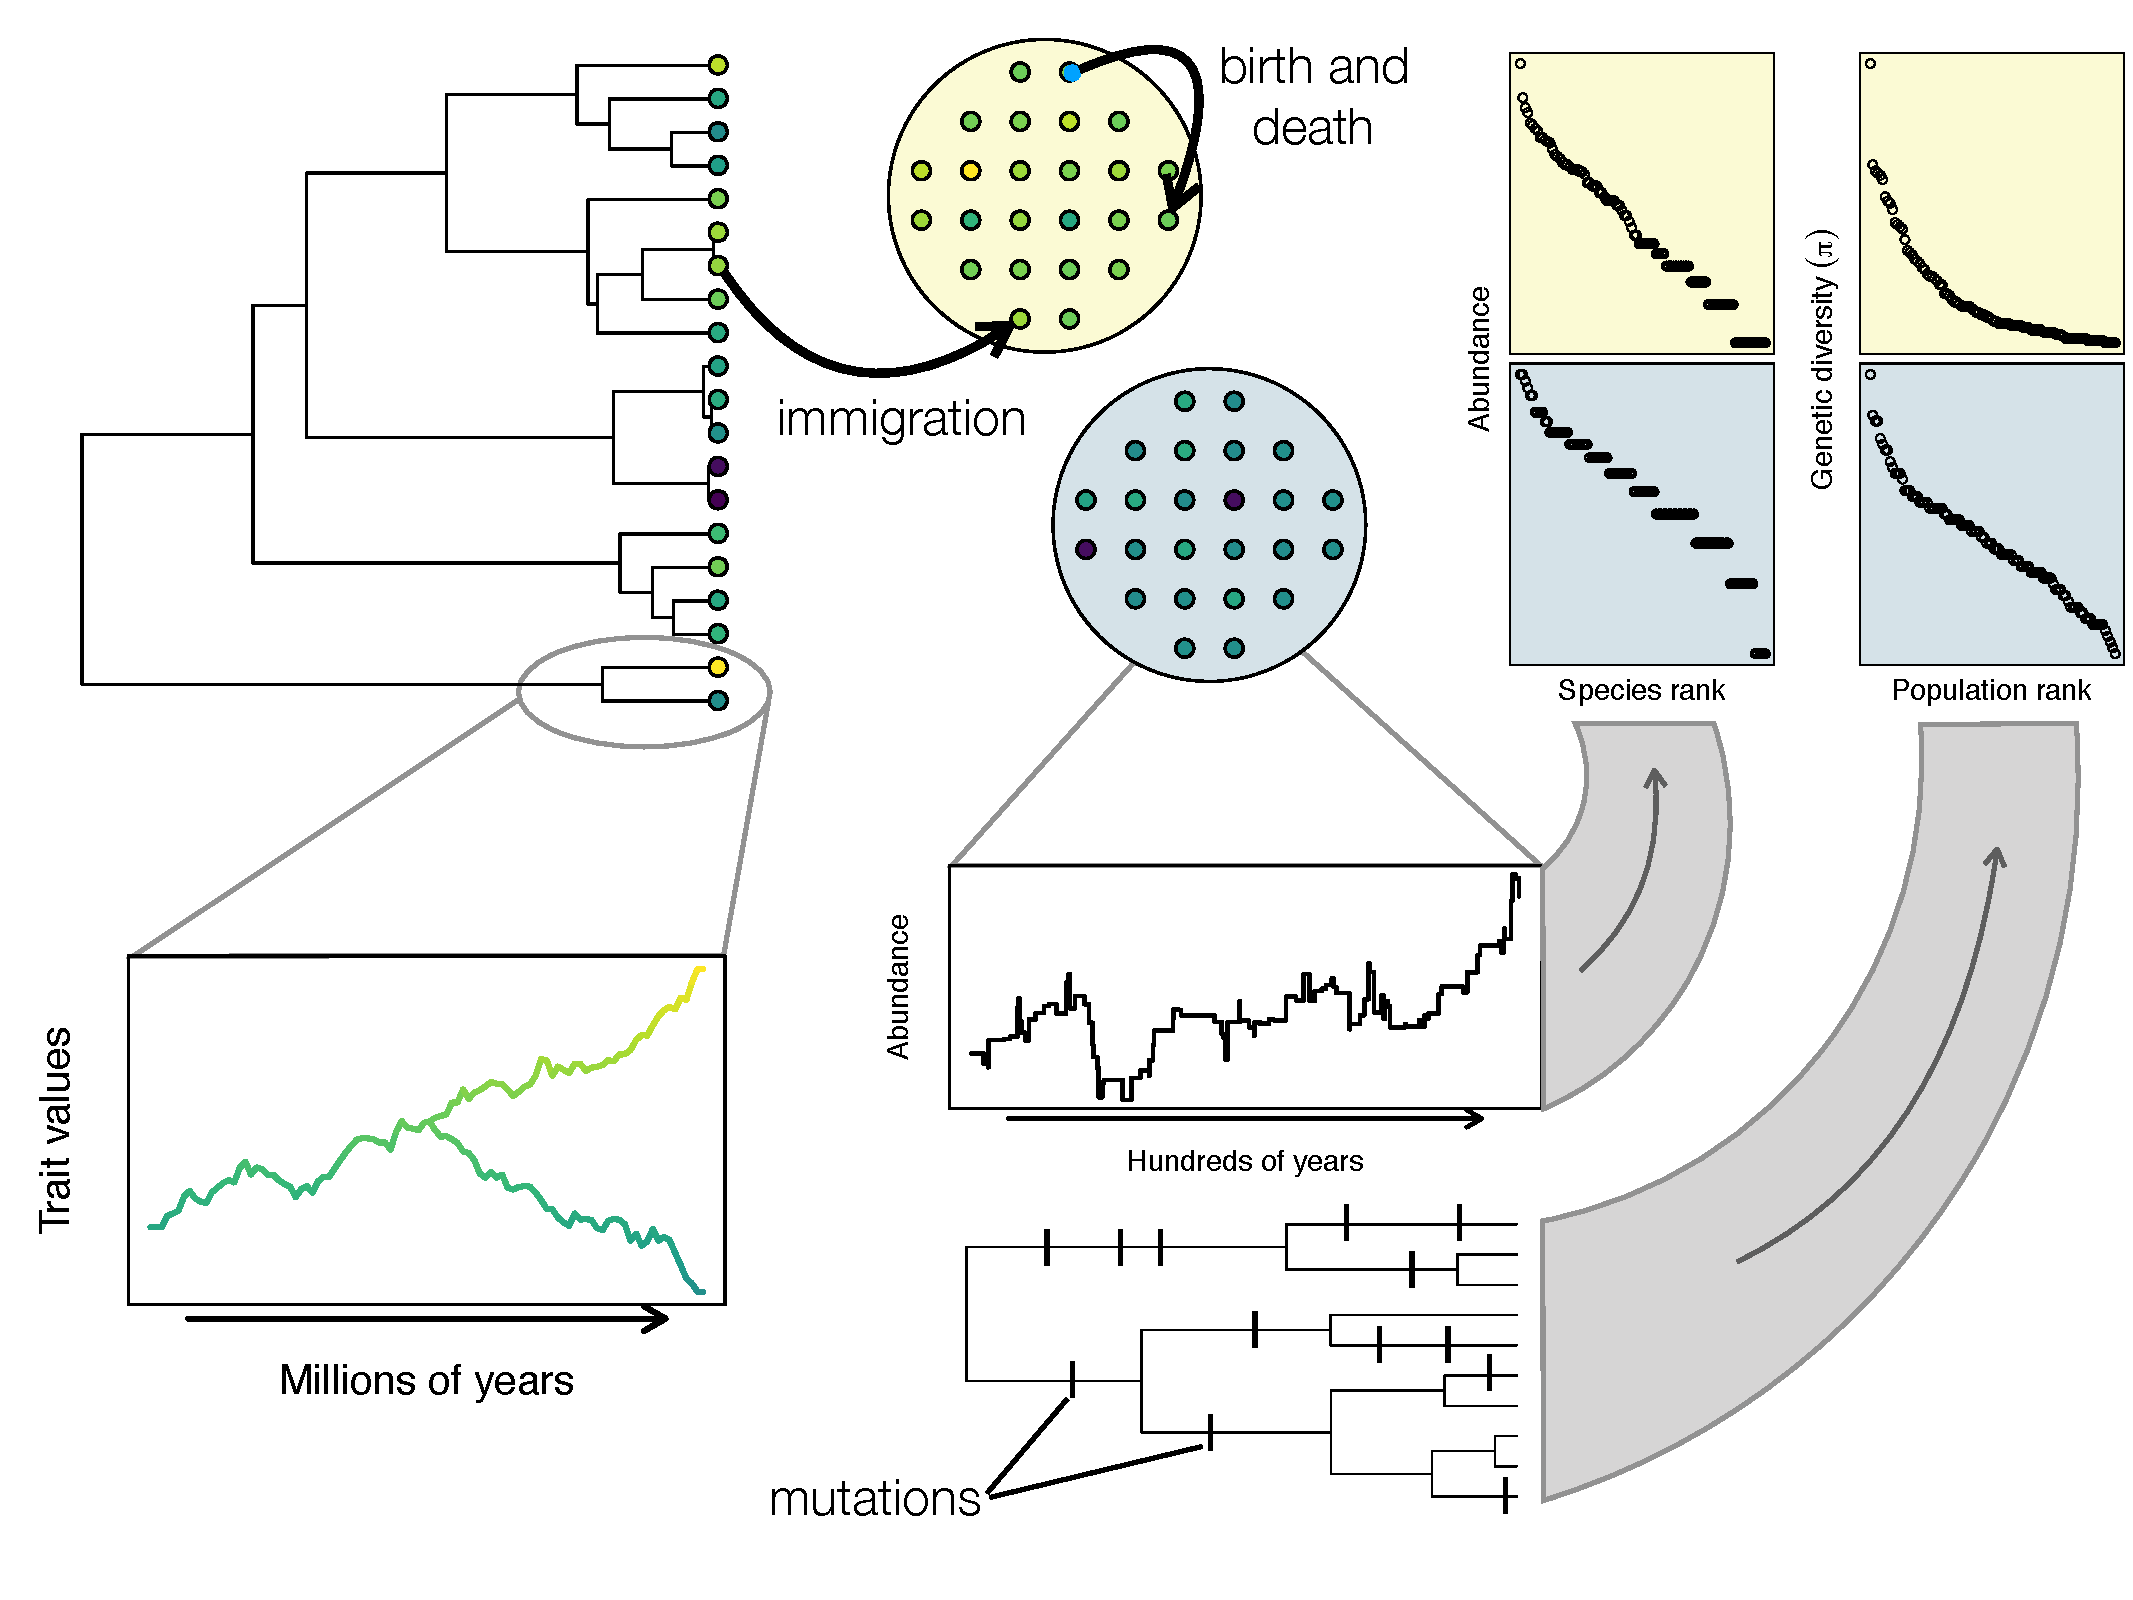
\includegraphics[width=0.7\textwidth]{../fig_mod.pdf}}
\end{figure}

% \begin{figure}[htbp]
% \centering
% 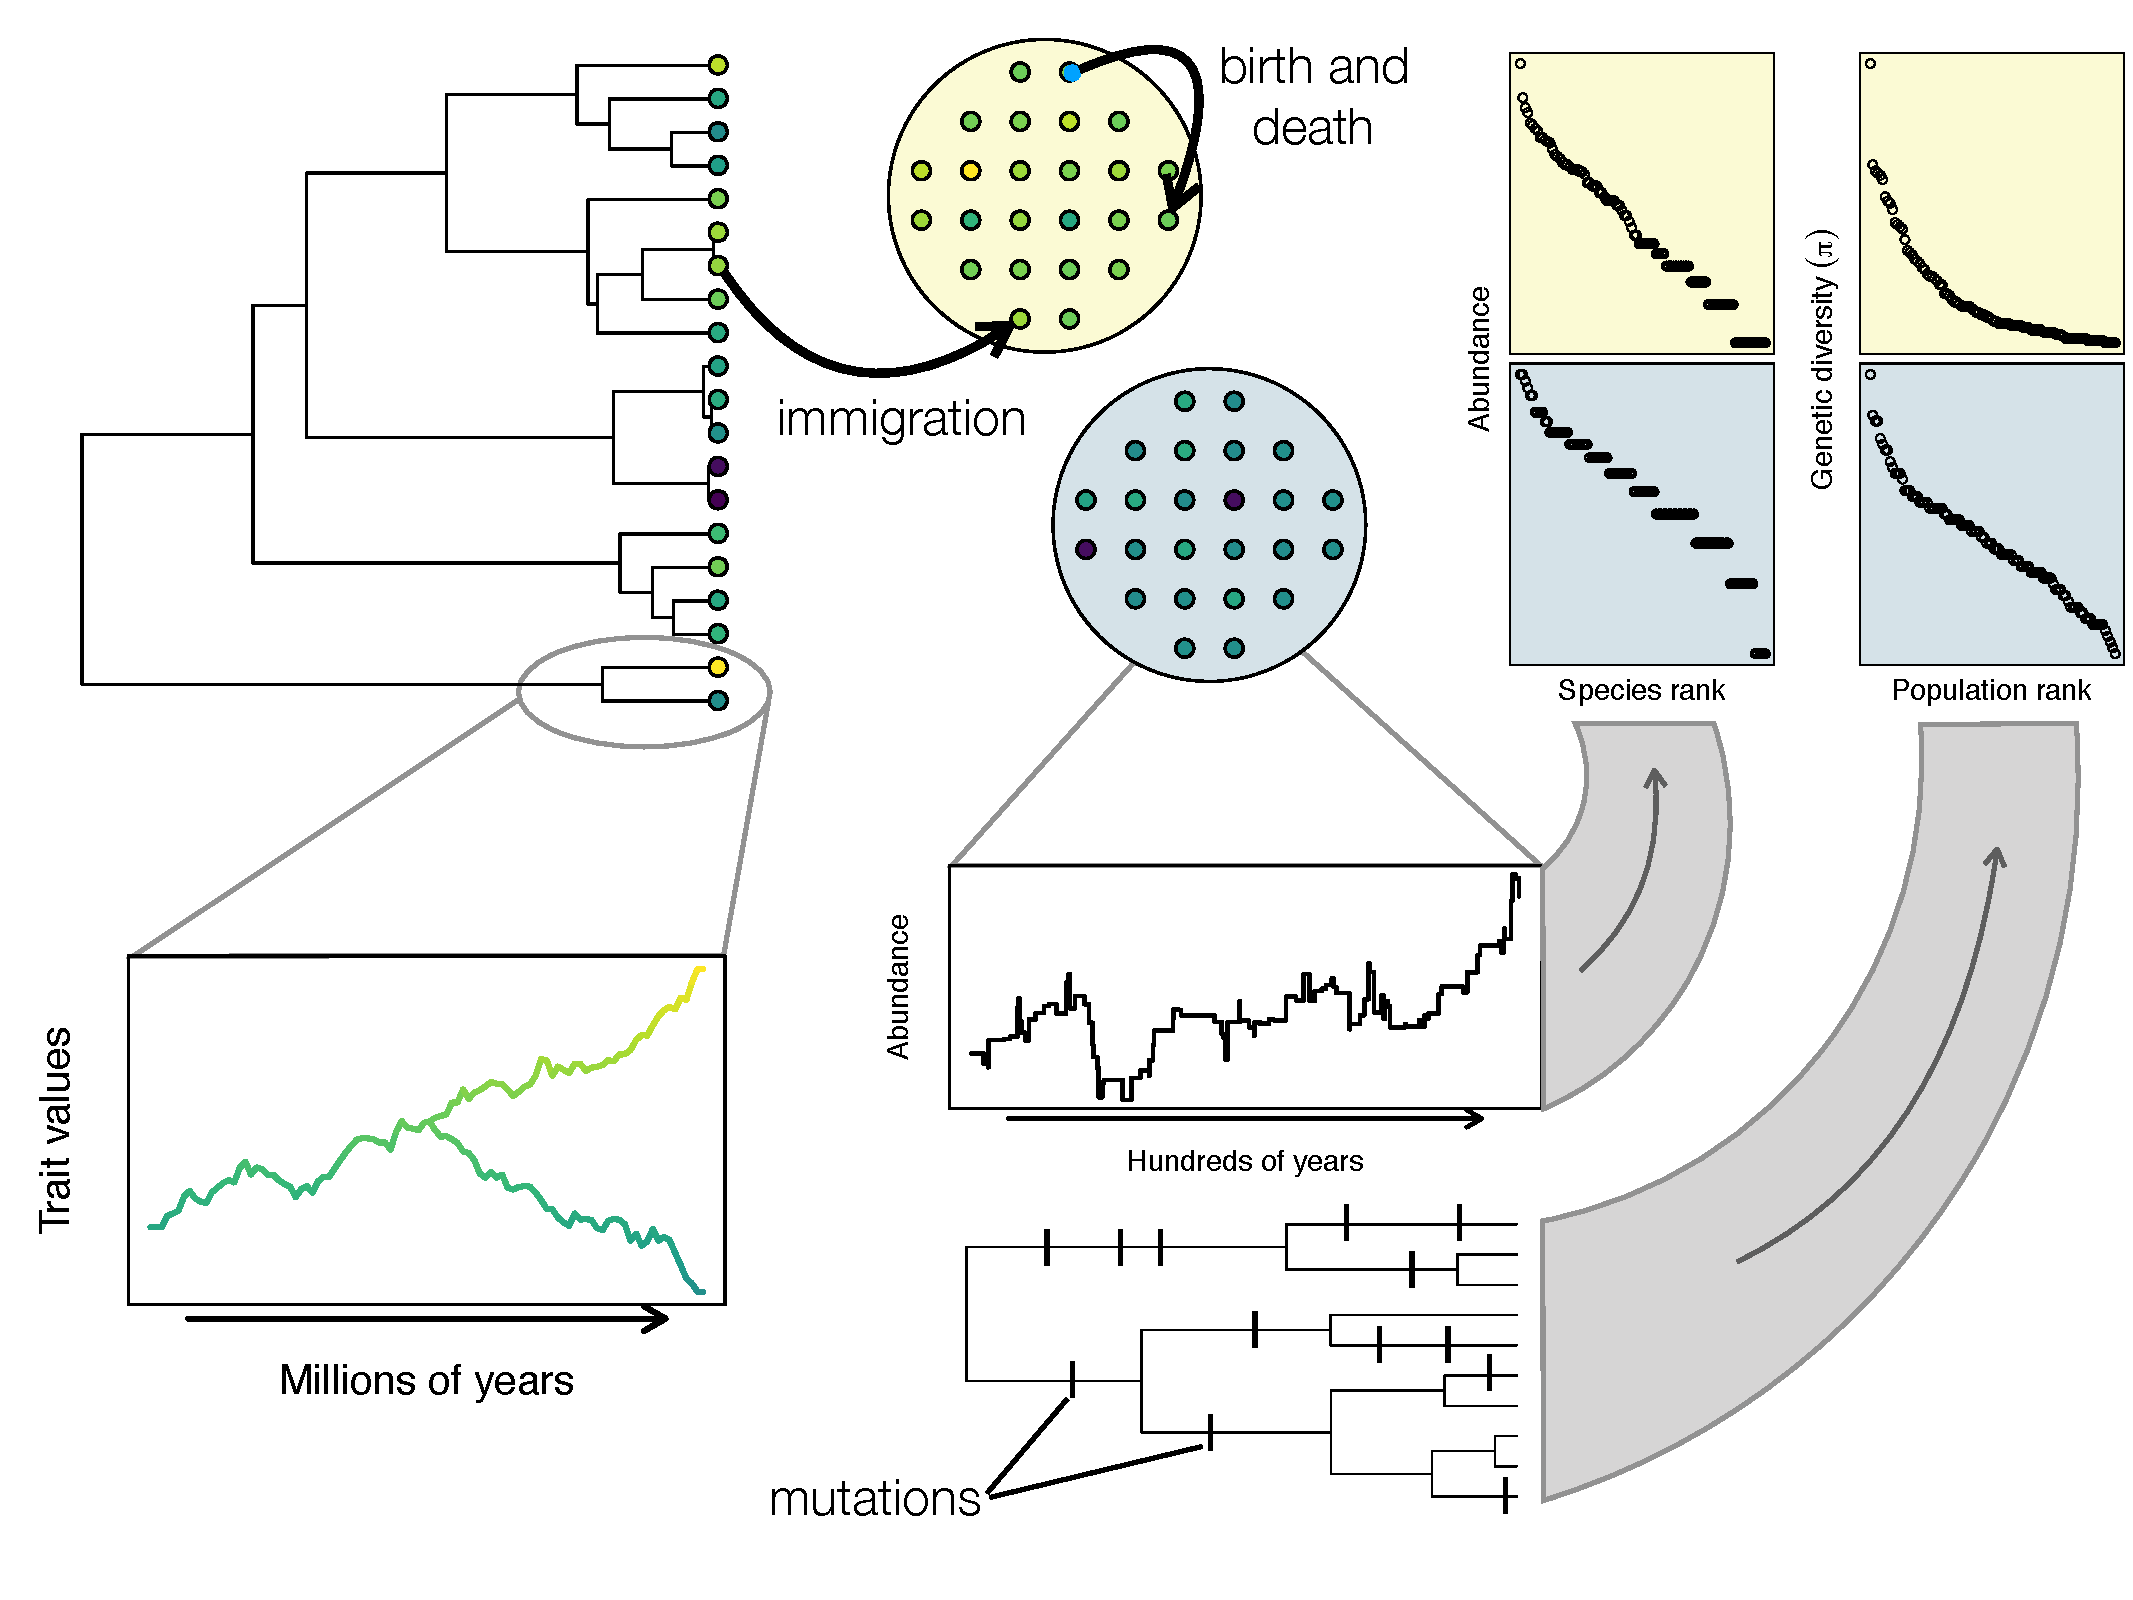
\includegraphics[width=0.7\textwidth]{../fig_mod.pdf}
% \caption{The processes captured by our model and the data types
% predicted. Colors correspond to trait values. The processes are: birth,
% death, immigration, and mutation in a coalescent framework (all of which
% operate primarily on short time scales), and speciation and trait
% evolution (all of which operate primarily on longer time scales). These
% processes may be modulated by trait-based interactions among species and
% between species and their environments as presented in Table 3.
% Different environments and their trait compatibility are illustrated for
% two hypothetical communities by the lighter background colors. The
% modeled processes generate the four data types predicted by the model:
% species abundance, population genetic diversity across species,
% phylogenetic relationships between species, and trait distributions
% across species.}
% \label{fig:mod}
% \end{figure}


\section{Proposed Research}\label{proposed-research}

\subsection{Research objectives and
hypotheses}\label{research-objectives-and-hypotheses}

We have three objectives:

\textbf{R1} To design and implement an informatics platform that can
synthesize and facilitate the sharing of diverse data streams associated
with DoB projects and similar biodiversity initiatives. We will make
this platform open source and usable both through a graphical user
interface and an R \cite{R_Development_Core2013-ze} package. We will
implement it across the five DoB projects represented by co-PIs on this
current proposal (Hawaii: Rominger and Gillespie; Palau: Dawson;
US-China: Soltis; Amazonia: Guralnick and Owens; Atlantic Forest:
Carnaval and Hickerson).

\textbf{R2} To build a joint model for the multiple dimensions of
biodiversity---species abundance, genetic, and functional. This model
will build off on-going work (by Rominger, Hickerson, Harmon, and Chase)
to combine macroecological predictions with phylo- and population
genetic measures. Model fitting methods based on ABC and machine
learning will be created. The entire modeling framework will be released
as open source software.

\textbf{R3} To test this joint model across five diverse systems for
which data has been synthesized by the informatics platform from
existing DoB sampling efforts and selective resampling. We have included
in this proposal five mature DoB projects whose data represent
compelling unit tests for our informatics platform, and whose underlying
evolution and ecology will test the generality of our model. We have
identified data types (e.g.~abundance, genetic and/or trait data) where
new targeted sampling within these projects will greatly improve our
ability to test our model and document the raw diversity of life.

The modeling approach we develop in \textbf{R2} allows us to address
five hypotheses central to ecology and evolution at an unprecedented
quantitative caliber and grounded in data aggregated (\textbf{R1}) from
incredibly diverse systems (\textbf{R3}). Our approach casts these
complex hypotheses as clear correlations (see Fig. \ref{fig:hyp})
between the parameters of our model (Table \ref{tab:mod}) when fit to
data across systems. Because the model encapsulates a range of processes
and jointly predicts many data types, interrogating its behavior
represents a rigorous, multi-faceted test of hypotheses
\cite{McGill2003-sf,McGill2007-zd,Leibold2017-jv}.

\begin{figure}[htb]
\floatbox[{\capbeside\thisfloatsetup{capbesideposition={right,top},capbesidewidth=4cm}}]{figure}[\FBwidth]
{\caption{Correlations between inferred parameters (see Table
\ref{tab:mod}) of our model under the assumption that our five
hypotheses are true. In {\bf H5}, ``competition'' and ``immigration''
refer to communities inferred to be competition-driven versus
immigration-driven, respectively.}\label{fig:hyp}}
{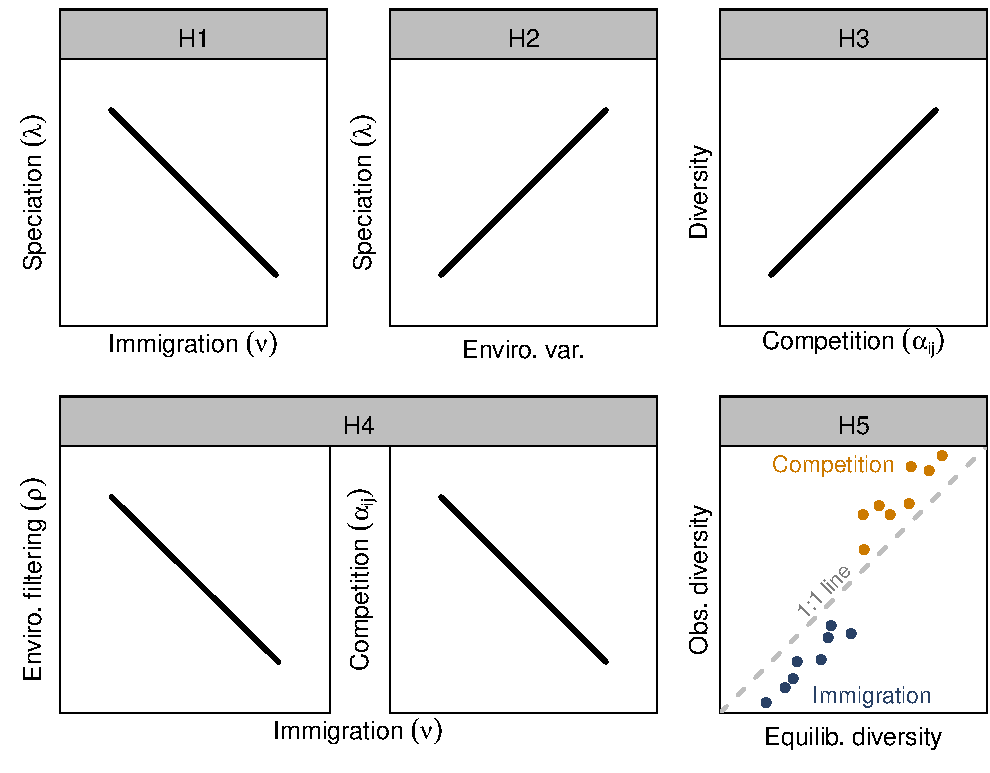
\includegraphics[width=0.7\textwidth]{../fig_hyp.pdf}}
\end{figure}

% \begin{figure}[htbp]
% \centering
% 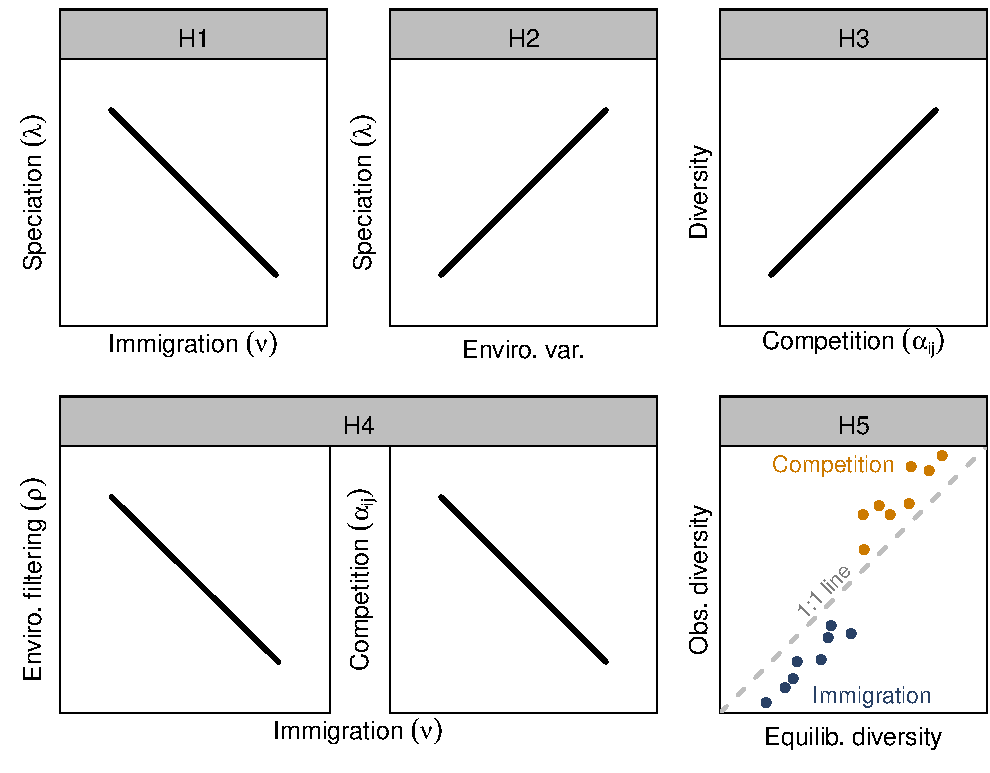
\includegraphics[width=0.7\textwidth]{../fig_hyp.pdf}
% \caption{Correlations between inferred parameters (see Table 3) of our
% model under the assumption that our five hypotheses are true.}
% \label{fig:hyp}
% \end{figure}

\textbf{H1: Isolation fosters diversification.} This has long been
assumed, documented empirically \cite{Losos2000-xp,Wagner2014-qm}, and
demonstrated theoretically \cite{Rosindell2011-od}. However, it remains
to be assessed whether isolation is key to the striking examples of
endemism and radiation at the species, genetic, and functional levels,
or if it is only secondary to other processes such as strong ecological
interactions. Looking across systems, this hypothesis predicts a
negative correlation between estimated immigration ($\nu$) and
speciation ($\lambda$; Fig \ref{fig:hyp}).

\textbf{H2: Environmentally-driven speciation is important across
  systems, but depends on intrinsic dispersal ability of taxa.}
Whether environmental gradients can promote diversification remains an
open debate \cite{Mittelbach2007-ui, Ogden2002-jb, Rundle2005-ll}. Our
model can test whether including interactions between traits and
environments is necessary to predict patterns of species abundance,
phylo- and population genetic diversity, and trait
distributions. After accounting for the effect of H1, this hypothesis
predicts a positive correlation between estimated speciation
($\lambda$) and the measured environmental heterogeneity of a study
region (Fig. \ref{fig:hyp}), which we can quantify spatially and
temporally for many studies.

\textbf{H3: High diversity systems result from increased strength of
  species interactions.} This is a classic hypothesis in the
latitudinal diversity gradient literature \cite{Pianka1966-ky} and
questions of ecosystem complexity and stability \cite{May1973-ua,
  Nuismer2013-wd}. If we find that high diversity systems are
systematically better-fit by models with strong trait-based species
interactions, this lends strong support to the hypothesis. Across all
systems, this hypothesis predicts a positive correlation between
diversity measured across all biodiversity dimensions and the
magnitude of estimated trait-based competition ($\alpha_{ij}$;
Fig. \ref{fig:hyp}).

\textbf{H4: Assembly by immigration (versus \emph{in situ} speciation)
  leads to weaker species interactions and thus more apparently
  neutral distributions of species abundances, genetic and functional
  diversity}.  If high diversity systems are the result of strong
species interactions, do these interactions arise more readily in
communities assembled by immigration or \emph{in situ} speciation? We
posit the latter, due to increased opportunity for co-evolutionary
arms race-like dynamics \cite{Quental2013-qv,
  ODwyer2014-gw}. Conversely, immigration-assembled communities will
draw from pools of the best, often most generalist, colonists and thus
appear effectively neutral. Thus, this hypothesis predicts a negative
correlation between inferred immigration and the magnitude of
parameters capturing purely non-neutral processes (i.e.~trait-mediated
interactions, both species-species {[}$\alpha_{ij}${]} and
species-environment {[}$r${]}; Fig.  \ref{fig:hyp}).

\textbf{H5: Most systems have not reached an equilibrium in
  diversity.}  Thus historical contingencies are critical for
understanding contemporary diversity. We posit that the mechanistic
importance of the previous four hypotheses is heightened by systems
being out of equilibrium. For systems in equilibrium, dynamical
processes can no longer be inferred, or their effect size will be
diminished \cite{Rabosky2009-gs}. The time to equilibrium, and whether
or not our model has reached it, is something we can quantify. We can
then continue running the model until equilibrium is reached. Across
systems we predict discrepancies between observed diversity across all
dimensions and the modeled equilibrium diversity
(Fig. \ref{fig:hyp}). Whether this discrepancy is toward higher or
lower observed diversity than equilibrium yields interesting
additional and complementary hypotheses that we will explore:

\begin{adjustwidth}{2.5em}{0pt}
\hspace{1.5em}\textbf{H5a} Systems constrained by immigration \citep[e.g.~arthropod
communities on young substrates in Hawaii;][]{Rominger2015-kb} will
show observed diversities lower than equilibrium.

\textbf{H5b} Systems driven by strong interactions will show diversity
overshoots in which non-equilibrium diversity is higher than equilibrium
diversity because interactions initially drive diversification beyond
the intrinsic carrying capacity of a system \cite{Gillespie2010-bv}.
\end{adjustwidth}

\subsection{Methods}\label{methods}

\subsubsection{Informatics pipeline}\label{informatics-pipeline}

Existing informatic platforms and metadata standards now only manage
subsets of the data we envision synthesizing: abundance and/or
occurrence, trait, genetic, and environmental. We identified major
barriers to creating this multi-dimensional biodiversity platform for
projects that span biogeographic regions as part of an NSF-funded
workshop on DoB data management (PIs Carnaval and Soltis). These
barriers are (1) allowing for short-term data entry and long-term data
storage and sharing; (2) integrating abundance, phylogeny, and
environmental data into a data management environment primarily
intended for specimen data; and (3) educating researchers about proper
data management. This last barrier we address with substantial
curriculum development, detailed in section
\ref{training-and-mentoring} on training and Broader Impacts.

It is critical to insure that trait, occurrence, and abundance data
are standardized properly across all projects. We will use
entity-quality relationships to standardize key traits shared across
the tree of life, namely body size and metabolic rate. Those traits
specific to groups will also be modeled using a similar approach. Both
individual and species-level traits will be synthesized following a
new relational data model developed by Co-PI Guralnick.  Abundance
data will be standardized using Humboldt Core \cite{Guralnick2017-xb}
which captures necessary inventory metadata. Efforts at standardizing
content will assure both model-ready data, and reproducibility and
re-use for others.

We will build an open source R package that allows users to manage and
synthesize their data via three cloud-based and/or open repositories:
(1) Google Sheets for data entry and short-term curation; (2) Amazon
Relational Database Services (RDS) for mid-term curation; and (3) open
repositories detailed below for long-term curation.

Data for such large initiatives as DoB projects necessitates that many
participants be involved in the collection and curation of data.
Cloud-based platforms are ideal for distributed data collection because
they can be accessed remotely and track the version history produced by
multiple users. To this end, Rominger, working with undergraduate
students in focused mentoring associations, has developed an open source
R package \cite{Rominger2016-mq} that facilitates the entry and error
checking of data using R and Google Sheets, either through custom
scripts or a graphical user interface (GUI) built with Shiny
\cite{RStudio_Inc2013-bt}. This approach will be extended to facilitate
the entry of data types including abundances, phylogenies, and raw
sequence data. For data that cannot be easily recorded in tabular format
(e.g.~phylogenies), links to those files will be recorded instead.

Once data entry is complete we will house data on Amazon RDS and provide
functionality in our R package and Shiny app for data transfer to Amazon
RDS. Amazon RDS provides a scalable solution that reduces administration
costs and provides a simple solution for access to content via query
APIs. It is also easy to connect to such databases via R
\cite{Wickham2015-cj}. We will assure open access to resources via R and
the Shiny app to team members and the larger community, thus hastening
increased re-use.

Solutions for open, long-term curation of all data types of interest to
our project have already been pioneered. The missing component is
practical software to link data from these repositories for a given
project. We will fill this gap by making our extended R package work not
only with Google Sheets, local files and Amazon RDS, but with the APIs
of data aggregators and curators. We will specifically target GBIF for
occurrence data \cite{Flemons2007-eg}, NCBI for sequence data
\cite{Sherry2001-pn,Benson1993-jf}, OpenTree for phylogenies
\cite{Hinchliff2015-vi}, Map of Life for abundance data
\cite{Jetz2012-uq,Guralnick2017-xb}, TraitBase for traits
\cite{Bartomeus2018-zq}, and GloBI for biotic interactions data
\cite{Poelen2014-lg}. Importantly, all these curation platforms already
have dedicated R packages
\cite{Chamberlain2014-ds,Winter2017-ei,Michonneau2016-yc,Molina2017-hm,Poelen2018-vp}
that interface with their APIs, which we will leverage for our newly
developed package. We will use these existing resources to create
high-level functions that facilitate the publishing of data from Google
Sheets, local files, and Amazon RDS to these open repositories. Again,
this functionality will be made available both as a standalone R package
and as a Shiny GUI.

To facilitate our specific data needs for testing our model of
eco-evolutionary community assembly, we need to be able to compile data
by three potentially overlapping ways, each targeting specific shared
attributes across disparate data types to merge---or ``join''---relevant
information from all data types. We will use a PostgreSQL
\cite{Douglas2003-zs} backend in our R package to allow for these three
joins:

\begin{enumerate}
\def\labelenumi{\arabic{enumi}.}
\item
  Spatial joins: we must be able to collect all relevant data, from
  occurrences, abundance, and environments, for a specific location or
  region.
\item
  Phylogenetic joins: we must be able to collect all relevant data for a
  clade defined by a sample of its constituent members
\item
  Data availability joins: we must be able to identify clades and
  regions for which sufficient data are available and then collate those
  data.
\end{enumerate}

These joins will allow us to, for example, find all taxa that have
abundance data at a given location, query their trait values which may
have been measured from specimens at different locations, compile a
phylogenetic tree for those taxa and the files containing their raw
sequence data.

\subsubsection{Collection of new data} \label{collection-of-new-data}

Because we selected five mature DoB projects, many data resources are
already available; our new data collection efforts will focus on
filling specific gaps (see Table \ref{tab:data}) to ensure continuity
of data types across projects.

\begin{table}[!htb]
\newcolumntype{M}[1]{>{\raggedright\centering\let\newline\\\arraybackslash\hspace{0pt}}m{#1}}

\definecolor{yes}{rgb}{0.63, 0.73, 0.9}
\definecolor{no}{rgb}{0.9, 0.79, 0.63}
\definecolor{planned}{gray}{0}

\newcommand{\yes}{\cellcolor{yes}}
\newcommand{\no}{\cellcolor{no}}
\newcommand{\planned}{\cellcolor{planned}}

\newlength{\dc}
\setlength{\dc}{0.08\textwidth}

\centering
  \footnotesize
  \begin{tabular}{|ll|M{\dc}|M{\dc}|M{\dc}|M{\dc}|M{\dc}|M{\dc}|}
    \hline
    {\bf Project} & {\bf Taxon} & {\bf Abund.} & {\bf Occur.} & {\bf Pop. gen.} & {\bf Phylo.} & {\bf Traits} & {\bf Enviro.} \\
    \hline \hline
    Hawaii & Arthropods & \yes & \yes & \yes & \planned & \planned & \yes \\
    \cline{3-8}
    Palau & Algae & \yes & \yes & \yes & \planned & \yes & \yes \\
    \cline{3-8}
    Palau & Invertebrates & \yes & \yes & \yes & \planned & \yes & \yes \\
    \cline{3-8}
    Palau & Fish & \no & \yes & \yes & \yes & \yes & \yes \\
    \cline{3-8}
    Atlantic Forest & Plants & \yes & \yes & \planned & \planned & \planned & \yes \\
    \cline{3-8}
    Atlantic Forest & Butterflies & \yes & \yes & \planned & \planned & \yes & \yes \\
    \cline{3-8}
    Atlantic Forest & Herpetofauna & \planned & \yes & \yes & \planned & \yes & \yes \\
    \cline{3-8}
    Amazonia & Plants & \planned & \yes & \yes & \yes & \planned & \yes \\
    \cline{3-8}
    Amazonia & Birds & \planned & \yes & \yes & \yes & \yes & \yes \\
    \cline{3-8}
    US-China & Plants & \yes & \yes & \yes & \yes & \yes & \yes \\
    \hline
  \end{tabular}

  \caption{Data resources available, and planned collection of new
    data. \textbf{\textcolor{yes!50!Blue}{Blue cells}} correspond to
    sufficient existing data, \textbf{\textcolor{no!60!Mahogany}{tan cells}}
    correspond to data gaps that will not be filled, \textbf{black cells}
    represent new data to be collected by this proposed project.}
\label{tab:data}
\end{table}

Gap-filling field work will complement our abundance, phylogenetic and
population genetic, and trait sampling. Our primary source for
choosing sites will be the experience of the PIs and the knowledge of
local collaborators, supplemented with information from satellite
images and remote sensing data. Below we detail the status of specific
projects, and what new data are needed to build robust phylogenies,
document the multiple dimensions of biodiversity, and test our model.

\textbf{Hawaii}. This project uses the dynamic geomorphology of the
Hawaiian Islands to examine the evolution of entire communities of
arthropods over extended time. A combination of community ecological
approaches with genomics of select evolutionary lineages allows us to
determine the importance of changing functional roles of taxa within
communities as they differentiate and assemble, and the role of that
dynamic community in fostering diversification. Currently missing from
this effort, and necessary for the model, are complete data on
functional traits and phylogenetic relationships. Body size data
already exist for $\approx 10^6$ specimens and trophic interactions
exist for a much more limited subset, namely herbivorous hemipterans
\cite{Rominger2015-kb}. We will add trophic interactions for all
herbivorous insects following the methods in Rominger et al
\cite{Rominger2015-kb}, as well as more general trophic position
(e.g.~predator, parasitoid, etc.) for all arthropods. In addition,
collaborator Boettiger is compiling trophic interaction data for the
Hawaii DoB based on field observations and sequencing of gut contents.
Genetic resources are quickly accumulating for the Hawaii project
following novel new metabarcoding practices
\cite{Krehenwinkel2017-zk}. We will augment these data, which provide
sequences from a single marker for all specimens, with multi-locus
sequencing for targeted voucher specimens in order to construct a
robust tree for $\approx 2000$ Hawaiian arthropod species
($\approx 100$ of which we will add through this grant). This will be
the first time such a mega tree has been constructed for Hawaiian
arthropods, many of which have never been phylogenetically treated at
all.

\textbf{Palau}. Extensive abundance and trait data (including body
size, trophic position and habitat preference) have already been
collected. This system also has an aggressive COI barcoding initiative
covering all invertebrates found (459 vouchered species and subspecies
in 205 genera). We will again use multi-locus sequencing of targeted
vouchers representing $\approx 100$ genera to build a comprehensive
phylogeny for invertebrates in Palau's unique marine lakes, augmenting
$\approx 1200$ barcoded samples. We will additionally analyze ancient
COI barcode eDNA using myBaits target capture from downcore sediments
followed by Illumina HiSeq sequencing to reconstruct community
composition and dynamics including the immigration or origination of
new alleles through time. A total of 75 m of cores span the Holocene
in 6 lakes, and are in storage at the LacCore facility (U. Minnesota).

\textbf{Atlantic Forest}. We will focus on amphibians ($> 100$ Hylidae
tree frogs within Boana, and the Phyllomedusinae), lizards (within the
Ecpleopodinae), butterflies ($\approx 50$ species in the Biblidinae
subfamily and the satyroide clade), and plants ($\approx 200$ species
within the Miconiae, 50 within the Bignoniaceae). For these groups,
data on geographic occurrence, population genetics, phylogenetics, and
functional traits already exist or can be straightforwardly gathered
or enhanced with strong involvement of CUNY undergraduate students and
the help of Brazilian collaborators. A backbone multi-locus phylogeny
already exists for these groups, but we will add $\approx 100$ each to
vertabrates and plants to increase the completeness and resolution of
those tree. To ensure completeness of the data table, we will generate
barcode data for all available and yet unsequenced individuals of the
target groups, following standard protocols \cite{che2012,
  Krehenwinkel2017-zk, bi2018chloroplast}. For the amphibian data, a
strong barcoding effort is in place already.  The primary information
gap in the Atlantic Forest are curated data quantifying abundance. To
address this, we will (1) merge and curate abundance inventories
already available for plants (a table of abundance of woody plants is
available for $> 20$ sites), butterflies (7 sites, available through
collaborator Freitas), amphibians and reptiles (5 sites, collaborator
Rodrigues); (2) complete five replicate surveys to complement the
vertebrate abundance data, covering both lowland and montane areas of
the forest; and (3) compile data on the history of biocollections for
these groups to build a model of occupancy from existing occurrence
data. These spatially broad occupancy estimates can be combined with
the spatially narrow but detailed abundance data and used in our
modeling framework.

\textbf{Amazonia}. We will focus on birds and two plant
lineages--Lecythidaceae and Miconieae--for which the most complete
data exist. For the plants, we will compile publicly-available
abundance data from forest inventory plots
\cite{Lopez-Gonzalez2011-wr, Ter_Steege2011-yr, Rainfor2018-so} to
augment the detailed occurrence, genetic, and functional trait data
that have already been collected for this group. To make use of the
many other species inventoried in forest plots, we will also target
voucher specimens to generate new sequence data that can be added to
existing resources for plant community phylogenetics
\cite{webb2008phylocom, Harmon2013-wb}.  For birds, we will perform
targeted mist-netting and point surveys to fill geographical and
taxonomic gaps in existing abundance data from museum records,
estimates from the eBird database, and long-term survey data provided
by co-PI Robinson and collaborator Loiselle.

\textbf{US-China}. The US-China project focuses on levels of diversity
across the classic eastern Asia-eastern North American floristic
disjunction. Detailed sampling of plant genetic, trait, and
phylogenetic diversity and soil and leaf microbial diversity at six
sites in eastern North America and 5 sites in China will be available
through the funded project; remote sensing data for 3 of the 6 North
American sites are also currently available. Each site is linked to
abundance data from NEON (US) and CERN (China) plots, with additional
abundance data for woody plants provided by the Forest Inventory and
Analysis Program (US Forest Service) and partner organizations in
China. We seek to collect sequence data for plant species and soil
microbes at four additional NEON sites in North America to improve
sampling across the large geographic and climatic gradient and to add
remote sensing data for additional NEON sites as the data become
publicly available. We will add trait data from publicly available
sources for any new species sampled. Occurrence data will be obtained
from public databases. Phylogenies for 30 plant genera from across the
disjunction will be completed in the funded project.


\subsubsection{Theory development}\label{theory-development}

Hickerson and his PhD student Overcast, who will be funded on the
current proposal, have extended the island-mainland neutral model
\cite{Rosindell2013-di} to include coalescence of alleles under
neutral mutation, thereby allowing joint predictions of species
abundance distributions (SADs) and population genetic metrics such as
genetic diversity ($\pi$). Rominger, Hickerson, Overcast, and
collaborators Harmon and Chase will extend this work further to
complete objective \textbf{R2} by including the process of speciation
\cite{Rosindell2010-gq}, the evolution of traits, and ecological
interactions (between species, and between species and their
environments) based on those traits. This work as initiated by a
working group between these researchers at the Santa Fe Institute, and
will continue to be independently fostered by working groups among
these researchers at German Centre for Integrative Biodiversity
Research.

Trait evolution will follow a continuous Markov process (see Table
\ref{tab:mod}) for continuous traits, and be thresholded
\cite{Felsenstein2012-aj} for discrete traits. Trait-environment
interactions will depend on the distance between an individual's trait
value and the optimal trait value for the environment, the greater the
distance the less the fitness of that individual. Trait-based
species-species interactions will be again based on the distance
between traits, in this case the closer the trait values of two
individuals, the stronger their Lotka-Voltera \cite{Wilson2003-kp}
competition. This full model (Fig. \ref{fig:mod}, Table \ref{tab:mod})
will jointly predict species abundance data, genetic and phylogenetic
data, and trait distributions.

Because available population genetic data across many individuals in a
community are limited to extremely reduced genomic regions, and often
mined for synonymous SNPs, we will initially model neutral mutations;
however, demography will be driven by potentially non-neutral ecological
dynamics, and thus population genetic measures, despite being
mutationally neutral, may still be far from the predicted drift-mutation
balance of a constant population.

Analytical solutions to such models might be available, but only in
the asymptotic limit of equilibrium \citep[e.g.,][]{Etienne2007-we,
  Rosindell2015-gp}. Because we are interested in potentially
non-equilibrial histories (hypothesis \textbf{H5}) as a driver of
biodiversity patterns, we will use efficient methods to simulate model
predictions under different scenarios (from neutral to trait-based
assembly) and use a combination of approximate Bayesian computation
(ABC) and machine learning methods to infer which models with what
specific parameter values are best supported by the data. Model
fitting is discussed in section \ref{model-fitting}.

Figure \ref{fig:mod} summarizes the simulation model which
incorporates two key time scales and spatial scales. Across short
timescales, slow rates of macroevolution and very large population
sizes render diversity at the largest spatial scale, the regional
pool, approximately constant. Abundances in the much smaller local
community fluctuate due to a birth-death-immigration process
\cite{Kendall1948-ri}, modified under the non-neutral models to
include trait-based interactions (Table \ref{tab:mod}).  The
fluctuating local population determines the effective population size
$N_e$ which, together with mutation rate, determines the distribution
of genetic diversities across species. Across long time scales new
species arise and traits evolve.

We will use well known mathematical results for assembly by birth,
death, and immigration \cite{Haegeman2017-kf,Kendall1948-ri} to
implement efficient forward time simulations.  These forward-time
assemblage histories will constrain the coalescent simulation of
genetic data \cite{Rosenberg2002-vb, waples2007}. We will use {\it
  msprime} \cite{Kelleher2016-an} to implement this coalescent
approach, which requires the time trajectory of effective population
sizes ($N_e$) for each species and the mutation rate $\mu$ as
input. The time trajectory of $N_e$ for a species is determined by
that species' simulated population fluctuations \cite{waples2007},
which in turn derive from the model parameters of birth ($b$), death
($d$), and immigration ($\nu$).  Mutation rate $\mu$ is also a free
parameter.

\subsubsection{Model fitting}\label{model-fitting}

All processes in Table \ref{tab:mod} are expressed by parameters which
need to be fit to data. Because we are interested in the
non-analytically tractable non-equilibrium dynamics of
eco-evolutionary community assembly (\textbf{H5}), we cannot derive
simplie likelihood functions, and so will use simulation-based
approaches to model fitting, including new advances in machine
learning and hierarchical ABC. Fitting our model that jointly predicts
four data axes that span the three dimensions of biodiversity under
many mechanistic processes is precisely the means by which we test our
hypotheses about the drivers of diversity (\textbf{R3}).

While ABC has been standard for inference of complex models
\cite{Beaumont2010-si}, we are also interested in exploring machine
learning approaches because they enable the efficient use of
high-dimensional data and parameters without specific knowledge of the
joint probability distribution. Unlike available ABC methods that can
become intractable in high-dimension applications with many summary
statistics, many supervised machine learning methods perform best in
such cases \cite{Anderson2014-fi,Breiman2001-ux}. As another strategy,
we will explore machine-learning Bayesian approaches that can use the
full data under a flexible Bayesian framework \cite{Chan2018-qh}, rather
than having to choose particular summary statistics.

For our ABC and machine learning approaches we will explore a range of
summary statistics that contain information from all four data axes
(species abundance, phylogenies, population genetics, and trait
distributions) while flexibly allowing some axes to be incomplete.
Incomplete data can be accounted for in two ways: (1) summary statistics
pertaining to the missing data can be masked, effectively integrating
over the possible values those data could take; or (2) a sampling model
can be added to allow for the inclusion of the sparse data that do
exist. The latter solution is particularly relevant when considering the
occurrence data available from many studies. In these cases, we will
simulate actual abundance data, but then coarse-grain those abundances
to occurrences according to a binomial sampling process with detection
probability $p$. Using such occupancy type models for occurrence data
is not unprecedented \cite{Tingley2009-kt}. However, in our approach we
will be able to even more accurately estimate $p$ because we will
augment studies with only occurrence data with actual abundance surveys.
Where occurrence points and surveys overlap in geographic regions, we
will be able to precisely fit the value of $p$, which then will be
carried by the model to all regions where occurrence data are available.

Based on preliminary work by Rominger, summary statistics based on Renyi
entropies (equal to the logarithm of the Hill number) of SADs in a
machine learning context can be as good or better than pure likelihood
approaches in parameter estimation. We will therefore begin with Renyi
entropies of SADs \cite{May2017-ji}, distributions of genetic
diversities across species, phylogenetic diversity \cite{Chao2010-oo},
and trait distributions as our summary statistics. We will evaluate
whether Renyi entropies are sufficient or if additional statistics
improve fit.

\subsubsection{Hypothesis testing}\label{hypothesis-testing}

Fitting our model to real data from diverse ecosystems will allow us
to understand whether a common set of mechanisms can be seen as
universally driving patterns of diversity (\textbf{R3}). By evaluating
how the best-fit model parameters vary across taxa and systems we will
test our five main hypotheses. Figure 3 shows how correlations among
estimated parameter values and between parameter values and intrinsic
characteristics of regions and taxa can confirm or refute our
hypotheses. Critically, not all systems are represented by the same
taxa, nor do they cover the same spatial scale. In searching for
correlations between model parameters we are prepared to
account for random effects of taxon and study.

Evaluating whether our five biogeographic regions have achieved
equilibrium (\textbf{H5}) requires added analytical nuance. For that,
we will take two approaches. In the case of Hawaii and Palau, the age
of ecosystems is knowable based on the geology of the system. We will
thus explore explicitly how the processes inferred by our model
themselves change through time, and how the community as a whole
approaches, but potentially does not reach, equilibrium. In the case
of Hawaii this is achieved by looking across the chronosequence
\cite{Rominger2015-kb}. In the case of Palau this is achieved by
looking explicitly at the sediment core from which we will extract
taxonomic, functional, and genetic data.

The proportion of equilibrium achieved
\citep[sensu][]{Rosindell2013-di}, will also be a parameter in our
simulation models (i.e.~it will determine for how long a given
simulation is run). By allowing this parameter to be fit to all our
datasets, not just those from Hawaii and Palau, we can understand
whether the community of interest has reached equilibrium. If we
estimate that it has not, we can then calculate what equilibrium
diversity would be under the best fit model. Comparing these
observations to the real data will allow us to understand whether the
non-equilibrium conditions produce higher or lower diversity across
the four data axes that map onto the three dimensions of biodiversity,
and whether the specific assembly process is predictive of diversity
overshoots or undershoots relative to equilibrium (\textbf{H5a-b}).

\section{Broader Impacts}\label{broader-impacts}

Our proposed project contributes to broader society in three quite
different ways: (1) training and mentoring in data science, including
specifically for underrepresented groups; (2) contributing open source
software for science and conservation; and (3) adding to the Tree of
Life.

\subsection{Training and mentoring}\label{training-and-mentoring}

We will work with Data Carpentry and Software Carpentry (``the
Carpentries'') to design new workshop content for heterogeneous
biodiversity data.The Carpentris are a non-profit organization that
teaches hands-on, evidence-based workshops. We will use our newly
developed content in a national workshop (for $\approx 30$
participants) to be hosted by the Co-PIs at the University of Florida,
who have demonstrated success in hosting such workshops. The data
science principles taught in the workshop will be practiced by
students---who will receive support to attend--- as they prepare,
curate, and publish the new data that will be generated for our
proposed research.

To make this educational material as broadly accessible as possible,
the biodiversity data science curriculum will be developed as a
massive open online course (MOOC) hosted on the Santa Fe Institute's
online education platform. This content will be licensed under
creative commons. The creation of this course will leverage existing
infrastructure and expertise at the Santa Fe Institute.

\subsection{Open source software for science and conservation}\label{open-source-software}

\subsubsection{Informatic platform}\label{informatic-platform}

We will provide open-source data management software that fills the
gaps of existing biodiversity data management and sharing tools,
developing a powerful and intuitive software that can help research
groups manage, curate, share, and publish their diverse data streams
associated with large, multi-dimension, multi-institution projects
exemplified by the DoB projects. This tool will also allow multiple
user experiences, from programmatic interface through an R package, to
a web-based graphical user interface enabled through Shiny apps.

\subsubsection{Eco-evolutionary synthesis
modeling}\label{eco-evolutionary-synthesis-modeling}

Our modeling framework, including simulations under different model
specifications, model fitting, and model selection, will be made
available as an open source R package.  With this modeling power at
hand, users will be able to gain completely new insights into their
study systems. Whether or not communities are assembled primarily by
in situ evolution or ex situ immigration strongly determines their
response to anthropogenic pressures \cite{Karp2012-is} and optimal
conservation management \cite{Barnosky2001-zy}. We will highlight this
importance in an open access applications manuscript which we will
seek to publish in a conservation-oriented journal. We will
specifically seek publicity for this work such that its message, and
our open source software, can be brought to the attention of
conservation practitioners.

\subsection{Adding to the tree of life} \label{adding-to-the-tree-of-life}

Expanding the Tree of Life is a community-wide priority, as we ought
to document diversity before human actions erase some of the most
remarkable realizations of the evolutionary process. The majority of
our data collection is aimed at adding robust tips to the Tree of
Life, complementing other ongoing projects \cite{Hinchliff2015-vi}.

\section{Timeline and Project Management} \label{timeline-and-project-management}

In the table below we detail the timeline for major milestones of our project.

\definecolor{Gray}{gray}{0.85}
\definecolor{gray2}{gray}{0.7}

\newcolumntype{M}[1]{>{\raggedright\centering\let\newline\\\arraybackslash\hspace{0pt}}m{#1}}
\newcolumntype{a}{>{\columncolor{Gray}}M{0.05\textwidth}@{}}
\newcolumntype{b}{>{\columncolor{white}}M{0.05\textwidth}@{}}

\renewcommand{\tabcolsep}{0pt}
\newcommand{\trule}{\rule[0ex]{1\linewidth}{1.5ex}}
\newcommand{\tline}{\arrayrulecolor{gray2}\hline\arrayrulecolor{black}}

\begin{center}
\footnotesize
\begin{tabular}{|m{0.005\textwidth} m{0.51\textwidth} | a b a b a |}
  \hline
  & Activity & Yr 1 & Yr 2 & Yr 3 & Yr 4 & Yr 5 \\
  \hline \hline 
  & Organizational working group at Santa Fe Institute (SFI) & \trule &&&& \\
  & Informatics pipeline & \trule & \trule &&& \\
  & Carpentries content hackathon & & \trule &&& \\
  & Carpentries workshop && \trule &&& \\
  & SFI MOOC development && & \trule && \\
  & Filling data gaps (abundance, genetics, traits) & \trule & \trule &&& \\
  & Model development & \trule & \trule & \trule && \\
  & Model validation and fitting with simulated data &&& \trule & \trule & \\
  & Model-based inference with real data &&&& \trule & \trule \\
  & Capstone workshop at SFI  &&&& & \trule\\
  \hline
\end{tabular}  
\end{center}


\subsection{Project Team Coordination} \label{project-team-coordination}

We have assembled a diverse team of researchers from theoreticians to
systematists to field ecologists. Rominger will lead coordinating
efforts across institutions remotely, and by bringing together the
group for logistical and synthesis meetings at the Santa Fe
Institute. Remote meetings will be held at least monthly to discuss
progress on independent tasks and on synthesis. Our larger group will
be organized into three core teams: (1) systems data gathering team,
(2) informatics team, and (3) theory development team. The
\textbf{systems team} will compile existing and collect new data from
our five biogeographic regions: Rominger and Gillespie (Hawaii),
Dawson (Palau), Carnaval and Michelangeli (Atlantic Forest), Owens and
Robinson (Amazonia), and Owens and Soltis (US-China)), along with
their collaborators. The \textbf{informatics team} (Rominger,
Guralnick, and Owens with support for a scientific programmer to be
housed at University of Florida) will coordinate with both the systems
and theory teams to build an informatics platform that satisfies both
groups' needs. The informatics team will also be responsible for
developing the biodiversity data science training curriculum in
collaboration with the Carpentries and the Santa Fe Institute Office of
Education. The \textbf{theory team} (Rominger, Hickerson, and
collaborators Chase and Harmon) will build our novel modeling
framework that jointly predicts species abundances, population and
phylo-genetics, and trait distributions. They will also coordinate
with the systems team to ensure the model's biological realism.

\section{Results from Prior Funding} \label{results-from-prior-funding}

\paragraph{Carnaval.} DEB 1343578: Dimensions US-BIOTA-Sao Paulo: A
multidisciplinary framework for biodiversity prediction in the Brazilian
Atlantic forest hotspot; 2013--2018; \$1,991,480. \textbf{Intellectual
Merits.} The team is developing models of spatial patterns of
biodiversity in the megadiverse Atlantic Forest of Brazil. They generate
and integrate: (1) environmental data from novel remote sensing-based
datasets and paleoenvironmental archives; (2) locality, phylogenetic,
genomic, and trait data from plants and animals; and (3) new methods
that incorporate big genomic and environmental data into predictive
models. The project has generated $80+$ publications to date,
including high impact journals
\cite{Do_Amaral2016-bi,Prates2016-at,Prates2016-gr,Maestri2016-bp,Zamborlini_Saiter2016-zu,Montade2016-wl,Bernal2016-pd,Bustamante2016-qt,Gu2017-oz}.
\textbf{Broader Impacts}. The project contributed to training of five
Ph.D.~students (2 female, 2 Latin-American), 11 M.Sc. students (10
female, 9 underrepresented minority), 7 undergraduates (all female/URM),
and 5 post-docs (2 female, 2 Latin-American).

\paragraph{Dawson. }OCE-1243970: Dimensions: Collaborative Research: Do
parallel patterns arise from parallel processes; 2013--2017 plus 1-yr no
cost extension; \$1,369,982\textbf{. Intellectual Merit}: We
investigated taxonomic, genetic, and functional diversity of microbes
and macrobiota in widespread yet under-explored marine lake ecosystems,
which present independent eco-evolutionary ``natural experiments.'' We
are revealing how parallel processes in space and time influence
genetic, phylogenetic, and functional diversity. We surveyed over 14000
points across 15 lakes in Palau, sampling 9000 specimens, and barcoding
1350 of invertebrates and algae. We are finding (1) marine lakes conform
with island theory, (2) microbes and macrobiota can share similar
biogeographic patterns, (3) abiotic lake dynamics are driven by regional
climate and local factors, and (4) life-history and chance strongly
influence population structure in invertebrates. Currently available
research products:
\cite{Dawson2016-zv,Dawson2016-aq,Meyerhof2016-fs,Schiebelhut2017-bp,Swift2016-iq,Wilson2017-en}.
Published datasets: BCO-DMO Project 2238 datasets. \textbf{Broader
Impacts}: 4 female graduate students (incl. 1 Pacific islander), 2
female lab techs, and a citizen scientist trained on the project.
Advised local resource managers on conservation.

\paragraph{Gillespie}: DEB 1241253 Dimensions: A community level approach
to understanding speciation in Hawaiian lineages. 2013--2019;
\$1,181,407. \textbf{Intellectual Merit}. This project aims to integrate
evolutionary and ecological theory to transform understanding of the
dynamics underlying community assembly. The synergy between the two
approaches is made possible through the use of a habitat chronosequence,
provided by the dynamic geomorphology of the young islands of the
Hawaiian archipelago. We selected 6 replicates in each of 12 sites and
are processing thousands of arthropod specimens while creating an mtDNA
barcode library and testing metabarcoding approaches. From these data we
are estimating macroecological metrics and conducting food web analysis.
For focal lineages, genomic data is providing information on population
differentiation over the island chronology. Papers to date:
\cite{Brewer2015-jo,Brewer2014-xc,Gillespie2013-mz,Shaw2016-aj,Gillespie2016-la,Gillespie2014-xm,Krehenwinkel2017-ea,Rominger2015-kb,Warren2015-zp,Yim2014-pr,Krehenwinkel2018-mz,Krehenwinkel2017-zk,Graham2017-su}.
\textbf{Broader Impacts}. Research is integrated into education; trained
9 postdocs, 10 graduate students, 44 undergraduates, and one high school
student.

\paragraph{Guralnick}: DEB-1262610: Collaborative Research: ABI
Development: Advancing Map of Life's Impact and Capacity for Sharing,
Integrating, and Using Global Spatial Biodiversity Knowledge; \$560,861;
2013--2018 plus one year no-cost extension. \textbf{Intellectual Merit}:
The Map of Life project focuses data integration based from a variety of
sources, including biocollections, species attribute data, expert
assessment of range boundaries, surveys, and inventories. This work
strongly enhances methods to publish, discover, openly link, and create
new knowledge, in order to further assessment of global biodiversity.
Papers to date:
\cite{Guralnick2007-yz,Guralnick2009-zu,Guralnick2010-gw,Jetz2012-uq,Parr2012-gh,Stucky2014-vb,Yilmaz2011-ll}.
\textbf{Broader Impacts}. The support has yielded web platforms that
provide data and knowledge and provided support for 2 Ph.D.~students.

\paragraph{Hickerson}: DEB 1253710: Career: Dynamic models of isolation and
admixture for community-scale population genomic inference; 2013--2017;
\$667,074 plus 1-yr no cost extension. \textbf{Intellectual Merits}.
Hickerson and colleagues developed inference methods to infer the
aggregate spatial history of species assemblages given genome-wide data
from multiple taxa. The grant has supported the publication of 22 peer
reviewed articles
\cite{Overcast2017-mf,Xue2017-hn,Emerson2015-tt,Myers2016-xu,Boehm2016-vu,Joseph2016-iu,Burbrink2016-ac,Brown2016-th,Prates2016-xv,Demos2015-px,Lipshutz2017-qq,Harris2016-oh,Alvarado-Serrano2015-zg,Xue2015-el,Emerson2015-xs,Boehm2015-ze,Robinson2014-ve,Robinson2014-vy,Smith2014-tb,Chan2014-nq,Demos2014-eu,Hickerson2014-za}\textbf{.
Broader Impacts}. The grant has supported two PhD students, two
postdocs, one undergraduate researcher who has gone on to pursue a PhD
in population genetics and an extensive educational outreach component.

\paragraph{Owens. }DBI 1523732: Postdoctoral Fellowship in Biology: Out of
the Tropics and Out of the Drawer: Integrative Analysis of the Tropical
Diversity Gradient from Museum Collections of New World Swallowtail
Butterflies; 2015--2017; \$138,000. \textbf{Intellectual Merit. }I
imaged and processed over 1300 butterfly specimens housed at four
institutions through a digitization pipeline I designed for this
project. Results, leading to one publication to date
\cite{Owens2017-ja}, suggest abiotic niche conservatism and
temperate-to-tropical dispersal are important, under-appreciated sources
of diversity in the tropics. \textbf{Broader impacts. }I engaged
worldwide volunteers through the Notes From Nature platform to
transcribe specimen label data. I have also participated in several
public outreach events at the Florida Museum of Natural history to
demonstrate how data derived from specimens can inform our understanding
of macroecology.

\paragraph{Soltis.} EF-1115210/DBI-1547229. Digitization HUB: A Collections
Digitization Framework for the 21st Century/iDigBio Phase 2;
\$12,661,986/\$15,486,747; 2011--2016 and 2016--2021.
\textbf{Intellectual Merit}. iDigBio is the national coordinating center
for digitization of biodiversity collections, the goal of which is to
make data for millions of biological specimens available in electronic
format. iDigBio currently serves over 108 million specimen records and
over 22 million media records, providing information on taxonomy,
geographic location, collector, date of collection, etc., and notes on
phenology, habitat, molecular resources, and other features, as well as
images and vocalizations. These diverse data promote integrative
biodiversity research, contain untapped trait data, and provide an
immense baseline for assessing impacts of climate change, invasive
species, and other environmental issues. The project has produced over
20 papers to date, including in \emph{Nature}, \emph{BioScience,
Proceedings of the IEEE International Conference on e-Science, New
Phytologist, Philosophical Transactions of the Royal Society B, American
Journal of Botany, Cladistics}, and \emph{ZooKeys}, among others
\textbf{Broader Impacts.} More than 100 workshops and hackathons have
fostered training in digitization workflows, use of digitized data in
research, applications in citizen science, education, and outreach.
Soltis has trained 2 post-docs, 6 graduate students, and 5
undergraduates.

%% suppresses bibliography, then make tex file to compile .bbl in separate doc
\bibliographystyle{grant}
\setbox0\vbox{\bibliography{dodoB.bib}}

\end{document}
